\begin{titlepage}
 
\begin{center}
 
 
% Upper part of the page
%
\includegraphics[width=0.7\textwidth]{jodcubelogo00}
%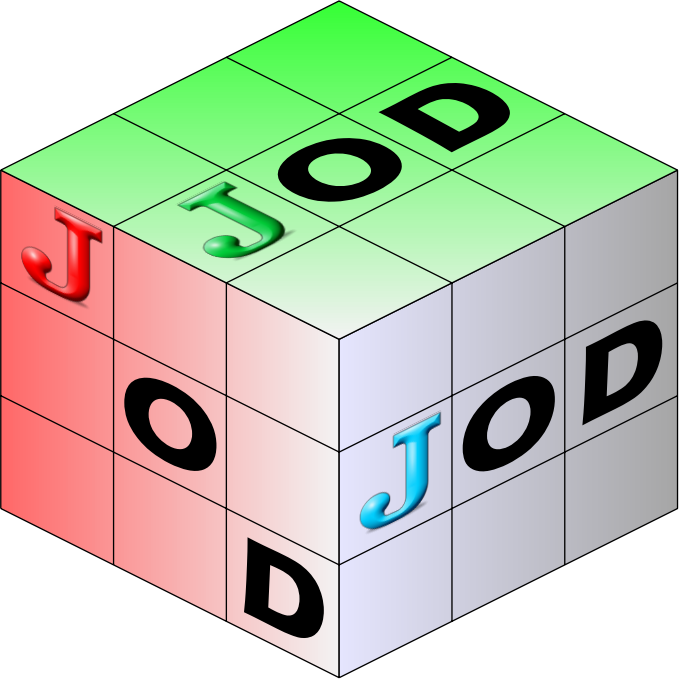
\includegraphics[width=0.7\textwidth]{jodcubelogo01} 
\href{https://bakerjd99.wordpress.com/the-jod-page/}{
\includegraphics[width=0.3\textwidth]{jodRGBcube}} 
 
% Title
\HRule \\[0.8cm]

{ \Huge \bfseries \jodred{J} \jodgreen{O}bject \jodblue{D}ictionary}\\[0.4cm]

\textsl{A code, test, and documentation refactoring addon for J}\\[0.4cm]
 
\HRule \\[0.8cm]
 
 
% Author and supervisor
\begin{minipage}{0.4\textwidth}
\begin{flushleft}
\emph{Author:}\\
John D. Baker \\
\texttt{bakerjd99@gmail.com} \\
\end{flushleft}
\end{minipage}
\begin{minipage}{0.4\textwidth}
\begin{flushright}
\emph{Release:}\\
\jodversion \\
\today \\
\end{flushright}
\end{minipage}

\vspace{0.8cm}

\emph{Print dimensions: US Letter}

Bound printed version at \href{https://www.amazon.com/dp/B08M2KBMND}{amazon.com} 

%\jodurl{https://www.amazon.com/dp/B08M2KBMND}
%\jodurl{http://www.lulu.com/shop/john-baker/jod-j-object-dictionary/paperback/product-20076023.html}
\href{https://www.amazon.com/dp/B08M2KBMND}{Amazon ASIN key: \texttt{B08M2KBMND}}

\begin{table}[ht]
  \centering
   \footnotesize
   %\rowcolors{0}{}{TableStripes}
   \begin{tabular}{|l|l|p{0.3\textwidth}|} \hline
      \multicolumn{3}{|c|}{\textbf{Document Version History}}\\ \hline
      \multicolumn{1}{|c|}{\textbf{Date}}  &
      \multicolumn{1}{c|}{\textbf{Version}} &
      \multicolumn{1}{|c|}{\textbf{Description}} \\ \hline\hline  
       \textbf{wip:} \today     & \jodversion        &  \\
       February 5, 2024    & 1.1.0       & j 9.52 update - hash sidecar files \\
       April 4, 2023     & 1.0.25        & j 9.42 update \\
       February 28, 2023     & 1.0.24        & j 9.41 update \\
       January 26, 2023     & 1.0.23        & j 9.04 $\beta$ update \\
       December 11, 2021 & 1.0.22       & direct definition update \\
       October 28, 2020     & 1.0.2        & Amazon edition \texttt{B08M2KBMND} \\
       March 28, 2020       & 1.0.1        & prior \texttt{pacman} release \\
       \ldots  & \ldots & \ldots \\ \hline
       \multicolumn{3}{|c|}{see: \jodurl{https://github.com/bakerjd99/joddoc}}\\ \hline
       \end{tabular}
	\caption{Abbreviated Document Version History}
	\label{tab:verhistory}
\end{table}
 

%\vfill 

% Bottom of the page
%{\large \today}
 
\end{center}
 
\end{titlepage}
